\documentclass{beamer}

\usetheme{MagdeburgFIN}
\usefonttheme{structurebold}
\usepackage{graphicx}
\usepackage{float}
\usepackage{url}
\usepackage{pdfpages}
\usepackage[ngerman]{babel}
\usepackage[utf8]{inputenc}


\title{Softwareprojekt - Android App}
\author{Gina Seckendorf, Alexandra Koch, Jonathan Kloss}
\date{24. Januar 2017}


\begin{document}

\begin{frame}[plain]
 \titlepage
\end{frame}


\section[Agenda]{}
\begin{frame}
\frametitle{Inhalt}
\tableofcontents
\end{frame}


\section{Idee}

	\subsection{Werwölfe von Düsterwald}
\begin{frame}
\frametitle{Ablaufdiagramm - Kartenspiel}
\includegraphics[width=\textwidth]{img/ad.jpg}
\end{frame}

	\subsection{Mehrwert}
\begin{frame}
\frametitle{Mehrwert}
\begin{itemize}
\item kein Spielleiter erforderlich!
\item intuitive Bedienung
\item Einsteiger-freundlich
\end{itemize}
\end{frame}


\section{Projektplanung}

	\subsection{Meilensteine}
\begin{frame}
\frametitle{Meilensteine}
\includegraphics[width = \textwidth]{img/ms.jpg}
\end{frame}

	\subsection{Projektplan}
\begin{frame}
\frametitle{Projektplan}
\vspace{0.3 cm}
\includegraphics[width = \textwidth]{img/projektplan.jpg}
\end{frame}

	
\section{Projektdurchführung}

	\subsection{Soll-Ist-Diagramm}
\begin{frame}
\frametitle{Soll-Ist-Diagramm}

[Soll 1 - Ist]

\end{frame}

\begin{frame}
\frametitle{Soll-Ist-Diagramm}

[Soll ... - Ist]

\end{frame}

\begin{frame}
\frametitle{Soll-Ist-Diagramm}

[Soll n - Ist]

\end{frame}

	
	\subsection{FINd die Werwölfe}
\begin{frame}
\frametitle{Klassendiagramm}
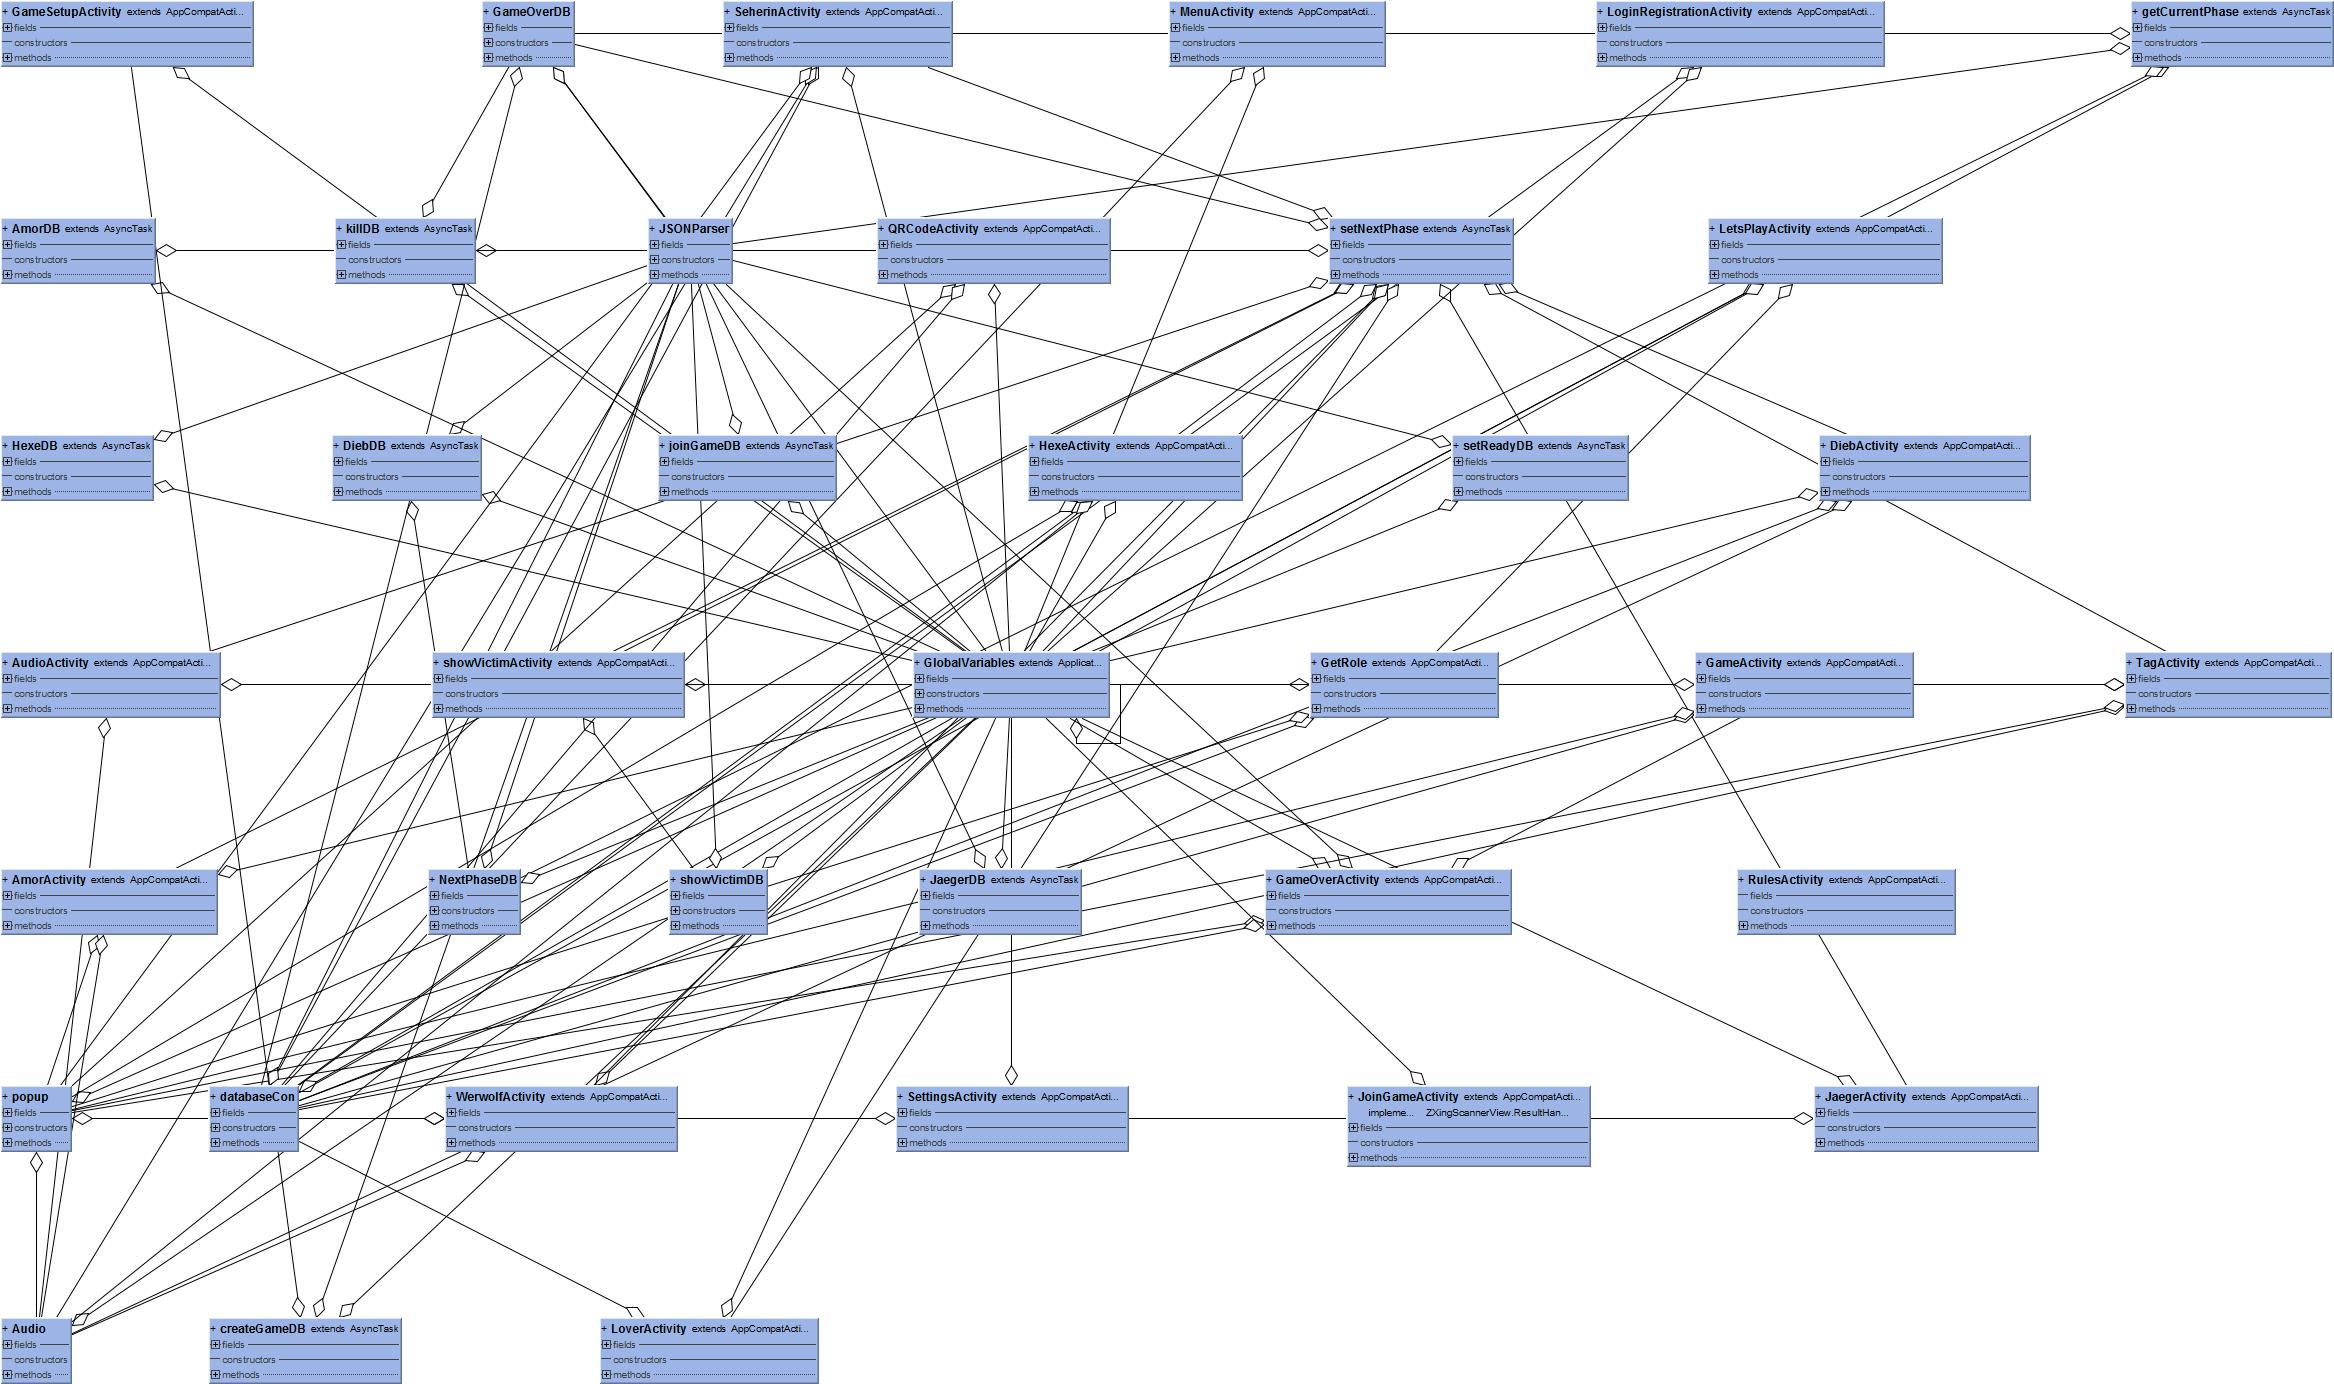
\includegraphics[width=1.0\textwidth]{img/WUML.jpg}
\end{frame}

\begin{frame}
\frametitle{Ablauf}
Screenshots; Erklärung ...
\end{frame}


\section{Projektbewertung}


	\subsection{Probleme}
\begin{frame}
\frametitle{Probleme}
\begin{itemize}
\item Umfang des Projektes einschätzen (sowohl Zeit- als auch Arbeitsumfang)
\\ $\rightarrow$ Einteilung der Arbeit
\pause
\item Kommunikation innerhalb des Teams
\end{itemize}
\end{frame}
	
	
	\subsection{Was haben wir gelernt?}
\begin{frame}
\frametitle{Lessons Learned}
\begin{itemize}
\item Bedeutung der Projektplanung
\begin{itemize}
	\item ausführliche Vorbereitung
	\item Aufgabenverteilung
\end{itemize}
\item ...
\item ...
\end{itemize}
\end{frame}


\begin{frame}
 \frametitle{Vielen Dank für Ihre Aufmerksamkeit!}
\end{frame}


\end{document}
